\section{Methodology}
\begin{figure}
    \centering
    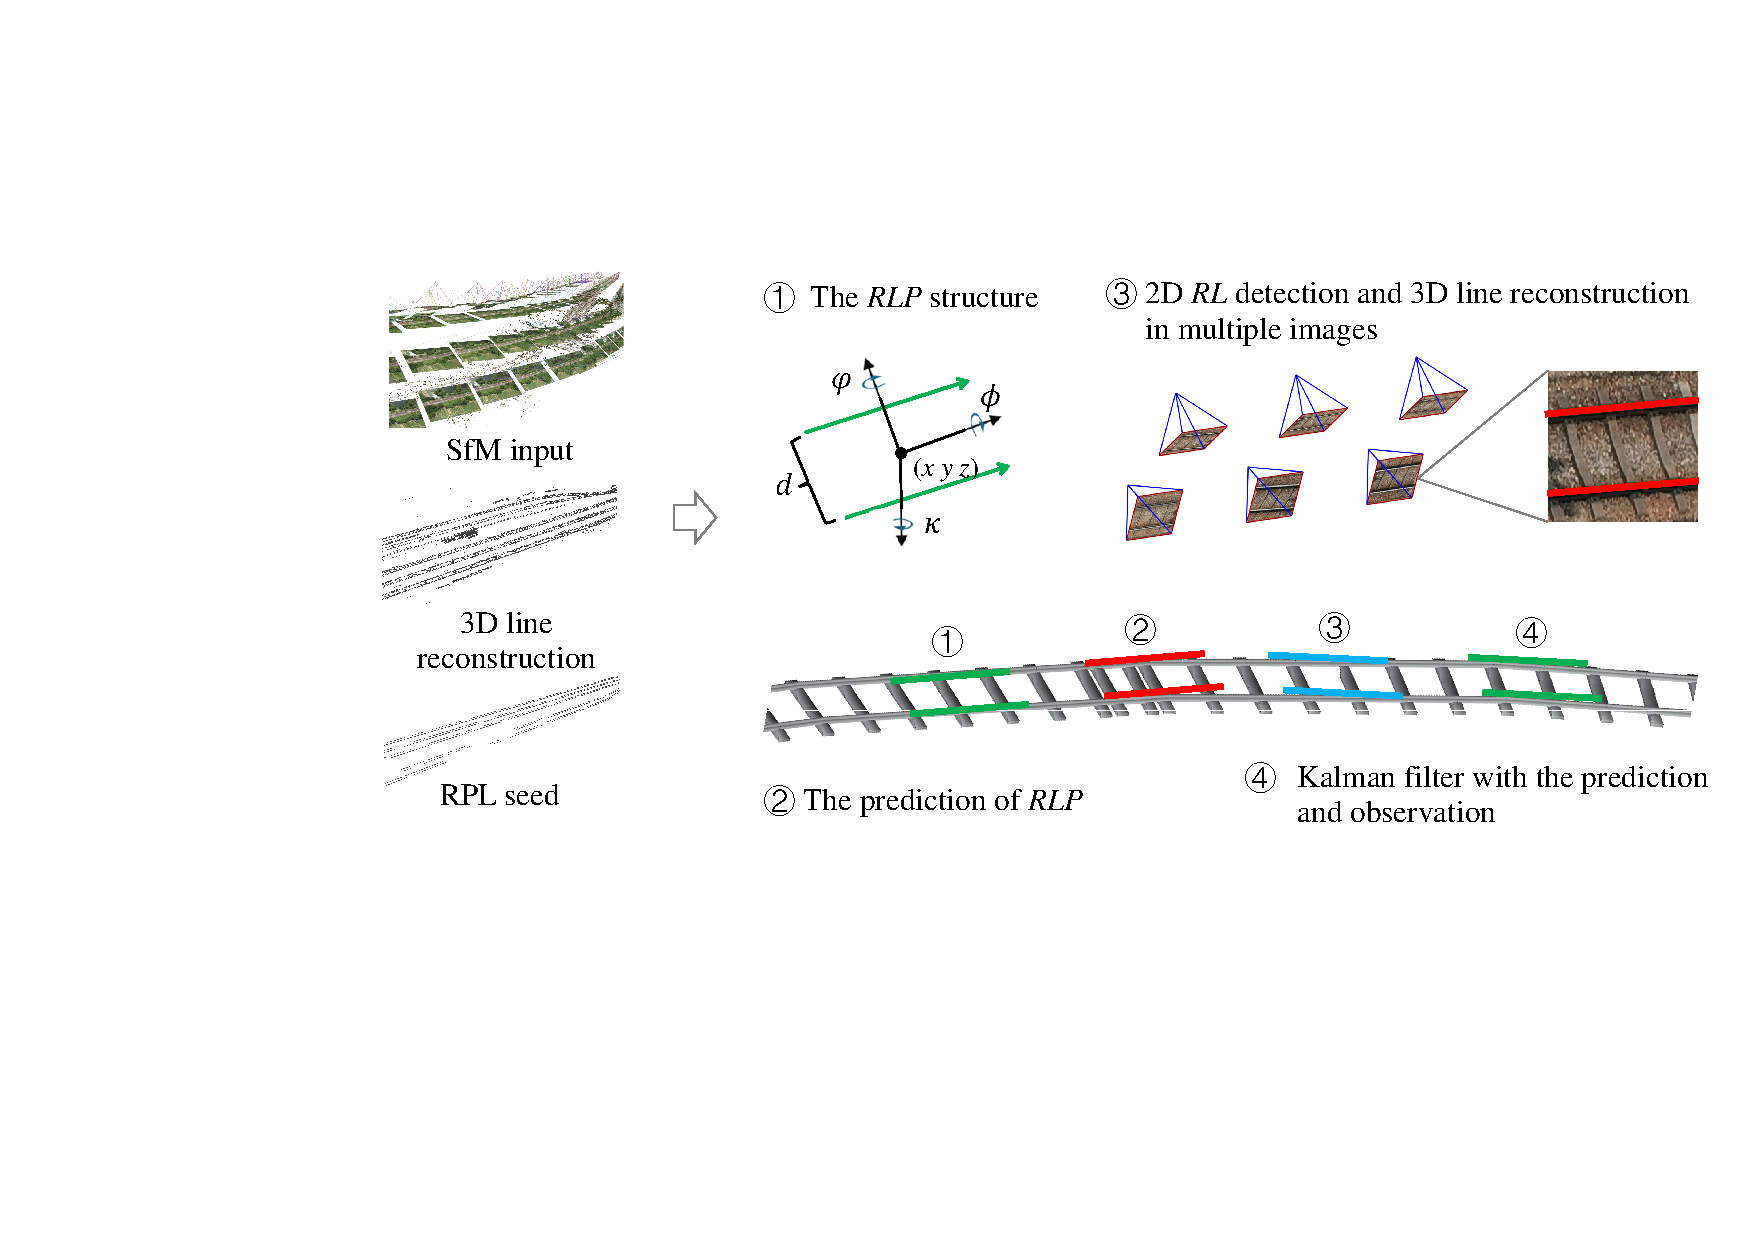
\includegraphics[width=0.98\textwidth]{images/overview.pdf}
    \caption{The flow of our method.
    It uses the aerial images as the input and produces accurate
    and connected 3D railway lines.}
    \label{fig_overview}
\end{figure}


The basic cell of our reconstruction is the railway line pair (\rlp) (\cref{fig_overview}~(1)).
An \rlp~consists of two railway lines (\textit{RL}) denoted as $D=\left\{L_i,L_j\right\}$.
The continuous \rlp~obtained in the Kalman process forms the \textit{RL} of the scene.
We use a center point $\left(x,y,z\right)$,
the position angle $\left(\phi,\omega,\kappa\right)$,
and the width $w$ of the two railway lines to shape the local \rlp:
\begin{equation}
\mathbf x = \begin{bmatrix}
    x,y,z,\rho,\kappa,\phi,\omega
\end{bmatrix}^ \top \in R^{7}.
\label{eq_prediction3} 
\end{equation}
Obviously,
$\mathbf x $ and $D=\left\{L_i,L_j\right\}$ can be converted into each other.

The flow of our method is presented in \cref{fig_overview}. 
It takes the SfM result of the aerial images as input.
We first obtain the 3D line with our 2D line extraction (\cite{ag3line}) and 3D line reconstruction (\cite{WEI2024}) algorithm.
Then
we cluster the single 3D line to find the seed of \rlp~ with the alignment in geometry and deep features (\cref{sec_initialseed}).
Starting with each seed,
we track and reconstruct the \rlp~in the framework of the Kalman filter (\cref{sec_kalman}),
in which the prediction and the observation come from the inner geometry of the \rlp~and the line reconstruction from multiple images,
respectively.


\subsection{Seed generation}
\label{sec_initialseed}
With the 3D lines $\left\{L\right\}$ reconstructed from \citep{WEI2024},
we first group the double lines of $L_i$ and $L_j$ as a seed candidate of the \rlp~  based on their angle $\theta$,
overlap $o$,
and projection distance $d$:
\begin{equation}
   \left\{D_i \mid \theta_{i1,i2} < t_\theta, o_{i1,i2} > t_o, d_{i1,i2} \in I \right\}.
    \label{eq_geometrycons}
\end{equation}
$t_\theta$ and $t_o$ are easy to choose
because the lines in \rlp~ are parallel and are highly overlapped;
while the interval of $I$ needs the rough width $\hat w$ of \rlp,
which can be acquired directly from construction standards or the measurement of point clouds.
We use one-third of $\omega$ as the margin error to reduce reliance on initial values,
i.e., 
$I=[\frac{2}{3}w,\frac{4}{3}w]$.
Because $L_i$ may satisfy \cref{eq_geometrycons} with many other lines,
we score $D_i$ by its geometry alignments to other candidates:
denote the central line of $D_i$ as $C_i$;
if the line segment distance between $C_i$ and $C_j$
is within $t_{dis}$,
the scores of both $D_i$ and $D_j$ are increased by the Gaussian weight:$\mathcal{N}\left(d_{i,j},0, t_{dis}/3\right)$,
where the first parameter is the line to line distance,
and the second and third parameter denotes the mean and the standard deviation,
respectively.
Then,
we sort the candidate of line pairs based on their scores and eliminate the pair whose 3D line has been grouped in the former pairs.

\begin{figure}[h]
    \centering
    \includegraphics[width=0.98\textwidth]{images/initialSeed.pdf}
    \caption{The initial seed with deep features.
    Given the line pair with geometry alignment, 
    we extract the deep feature for their image block in multiple image,
    with which we use the DBSCAN to confirm the initial seed of \rlp.}
    \label{fig_initialseed}
\end{figure}

Besides the geometry alignment,
the texture alignment of the \rlp~ is also employed to enhance the seed of \rlp.
As illustrated in \cref{fig_initialseed}, 
we acquire the image blocks for the line pair by the crop with their 2D lines.   
We project a line pair to at most four images where the two 3D lines induced,
which have been confirmed in the line reconstruction method \citep{WEI2024}.
To reduce the ambiguity of the texture feature caused by scale and rotation,
the local image is corrected to ensure that the center line of \rlp~ passes through the image center horizontally and the width of \rlp~ is half of the image.

We use the global average pooling layer in ResNet \citep{resnet} as the basic feature to describe the image block,
which has been trained on massive amounts of public dataset and can capture texture patterns for classification in the absence of labels.
Thus,
no additional benchmarks and training data are required in our method.
Denoting $\mathbf f \in R^n$ as the \rlp~ feature,
we acquire the set of features $\left\{\mathbf f_i\right\}_{i=1}^m$ from the image blocks.
Then,
we use DBSCAN to cluster the features with the cosine distance and retain the largest group as the seeds of the \rlp.
DBSCAN contains the parameters of the maximum distance between nodes and the 

\subsection{Railway track}
\label{sec_kalman}
Given the initial seed of \rlp,
we convert it to the form of $\mathbf x$ and take it as the starting place of a train.
We use the train's inertial forward direction for prediction,
during which the prediction $\bar{\mathbf x}$ in the next step is controlled by $\Delta t$ with the train's attitude:
\begin{equation}
        \begin{aligned}
            & x_k = x_{k-1} + \Delta t \cdot \cos(\phi_{k-1}) \cdot \cos(\omega_{k-1}), \\
            & y_k = y_{k-1} + \Delta t \cdot \sin(\phi_{k-1}) \cdot \cos(\omega_{k-1}), \\
            & z_k = z_{k-1} + \Delta t \cdot \sin(\omega_{k-1}),\\
            &\rho_k=\rho_{k-1},
        \kappa_k=\kappa_{k-1},
        \phi_k=\phi_{k-1},
        \omega_k=\omega_{k-1}.
        \end{aligned}
        \label {eq_statetransition}
\end{equation}
Note the train's attitude is unchanged in the prediction.
For each state,
there is an actual observation $\hat{\mathbf x}$ arising from the 3D railway line reconstruction in multiple images,
which will be discussed in \cref{sec_linereconstruction}.

The observation may contain errors induced from wrong 2D line detection and the corresponding 3D reconstruction,
and the prediction is easy to fail, especially when the train is passing through a bend.
Thus,
as shown in \cref{fig_kalmanflow},
we update the state of the train by combining the observation and prediction state with the discrete Kalman filter.
\begin{figure} [h]
    \centering
    \resizebox{0.98\textwidth}{!}{%
    \begin{circuitikz}
    \tikzstyle{every node}=[font=\normalsize]
    
    % 右侧矩形 (b)
    \draw [fill=gray!10,rounded corners=5pt]  (0,23.5) rectangle  
    node {\large
    \begin{minipage}{6cm}
    (b)~$\hat{\mathbf{x}}_k$ (\cref{sec_linereconstruction}) observation via
    3D line reconstruction.  
    \end{minipage}
    } (6.25,21.5);
    
    % 右侧矩形 (a)
    \draw [fill=gray!10,rounded corners=5pt] (0,20.5) rectangle  
    node {\large
    \begin{minipage}{6cm}
    (a)~$\bar{\mathbf{x}}_k$ prediction with \cref{eq_statetransition}
    and error covariance prediction via 
    \vspace{-0.5em}
    \begin{equation}
    \mathrm P_k= \mathrm F \mathrm {P}_{k-1}\mathrm F^{\top}+\mathrm Q
    \label{eq_xprediction}
    \end{equation}
    \end{minipage}
    }  (6.25,18.5);
    
    % 右侧大矩形,右移 0.5 单位
    \draw  [fill=gray!10,rounded corners=5pt] (8.0,23.5) rectangle  
    node {
        \large
    \begin{minipage}{7cm}
    (c)~Kalman gain update:
    \begin{equation}
    \mathrm K_k= \mathrm P_k 
    \left( \mathrm P_k +\mathrm R\right)^{-1}
    \label{eq_kalmangain}
    \end{equation}
    (d)~estimation update:
    \begin{equation}
    \mathbf{x}_k= \bar{\mathbf x}_k + \mathrm K_k \left(\bar{\mathbf{x}}_k- \hat{\mathbf{x}}_k  \right)
    \end{equation}
    (e)~error covariance update:
    \begin{equation}
    \mathrm P_k = \left( \mathrm{I} - \mathrm{K}_k \right) \mathrm P_k
    \end{equation}
     \end{minipage}
    } (15.5,18.5);
    
    % 拉长的右侧箭头
    \draw [->, >=Stealth] (6.25,22.5) -- (8.0,22.5); % 拉长到 8.0
    \draw [->, >=Stealth] (8.0,19.5) -- node[midway, above] {$k=k+1$} (6.25,19.5); % 拉长到 8.0 并添加标签


    % 左侧矩形 Initial estimate,左移 0.5 单位
    \draw [rounded corners=5pt] (-7.7,20.5) rectangle  
    node {\large
    \begin{minipage}{5cm}
    Initial estimation of $\mathbf {\hat{x}}_k$~(\cref{sec_initialseed}) and the initial covariance error $\mathrm P = \mathrm{I}_{7\times 7}$
    \end{minipage}
    } (-1.72,18.5);
    
    % 左侧矩形 Check for termination,左移 0.5 单位 []
    \draw [rounded corners=5pt] (-7.7,23.5) rectangle  
    node {\large
    \hspace{0.4em} 
    \begin{minipage}{5.5cm}
        \raggedright % 使标题顶格
        Check for termination:
        \vspace{-1em}
        \begin{itemize}
            \setlength{\itemsep}{0pt} 
            \setlength{\parskip}{0pt} 
            \setlength{\parsep}{0pt}
            \setlength{\leftskip}{0pt} % 保持item缩进
            \item non-convergence of reconstruction~(\cref{sec_linereconstruction})
            \item positional overlap 
        \end{itemize}
    \end{minipage}
    } (-1.72,21.5);

    % 拉长的左侧箭头
    \draw [<-, >=Stealth]  (0,19.5)-- (-1.72,19.5); % 左侧箭头延长到 -1.72
    \draw [<-, >=Stealth] (0,22.5)--(-1.72,22.5)  ; % 左侧箭头延长到 -1.72
    
    % 新增的箭头连接 (b) 和 (a)
    \draw [->, >=Stealth] (3.125,20.5) -- (3.125,21.5); % 从 (b) 底部到 (a) 顶部

    \end{circuitikz}
    }%
    \caption{The flow of Kalman filter for the \rlp~estimation. $\mathrm{Q}$ in \cref{eq_xprediction} and $\mathrm{R}$ in \cref{eq_kalmangain} represent the covariance matrix of observation noise and process noise, respectively.}
    \label{fig_kalmanflow}
\end{figure}

Because the transition is a nonlinear process,
we use the Jacobian matrix in \cref{eq_xprediction} for the linear transition of $\mathrm F_k \in R^{7\times7}$:
\begin{equation}
    \begin{aligned}
        &\mathrm F^k_{1:2,6:7}=\Delta t\left[\begin{matrix}
             -\sin(\phi_{k-1}) \cos(\omega_{k-1}) & - \cos(\phi_{k-1}) \sin(\omega_{k-1})\\
             \cos(\phi_{k-1}) \cos(\omega_{k-1})  & \sin(\phi_{k-1}) \sin(\omega_{k-1})
        \end{matrix}\right]\\
        &\mathrm F^k_{i,i}=1,i \in [1,7].
    \end{aligned}
    \label {eq_jacobian}
\end{equation}

For each seed of \rlp~,
we will track it with a Kalman filter toward two directions by setting a positive and negative $\Delta t$,
respectively.
Each track is terminated when one of the following two conditions is met.
(1) \textit{Overlap}:
a half of the nearest \rlp~is within $t_{dis}$ of the \rlp~that have been reconstructed in the previous filter process.
(2) \textit{Degenerate reconstruction:}
there is no correct 3D line that can be reconstructed from multiple images in \cref{sec_linereconstruction}.
Note that
it is unnecessary to check for termination in every estimate, 
especially when we use a small $\Delta t$ for robustness.
Instead,
we employ this check when a certain number of iterations are reached and roll back to the state of the previous check when the overlap or degenerate reconstruction occurs. 

\begin{figure}[htbp]
    \centering
    % 第一个子图
    \subfloat[Hough line detection]{
        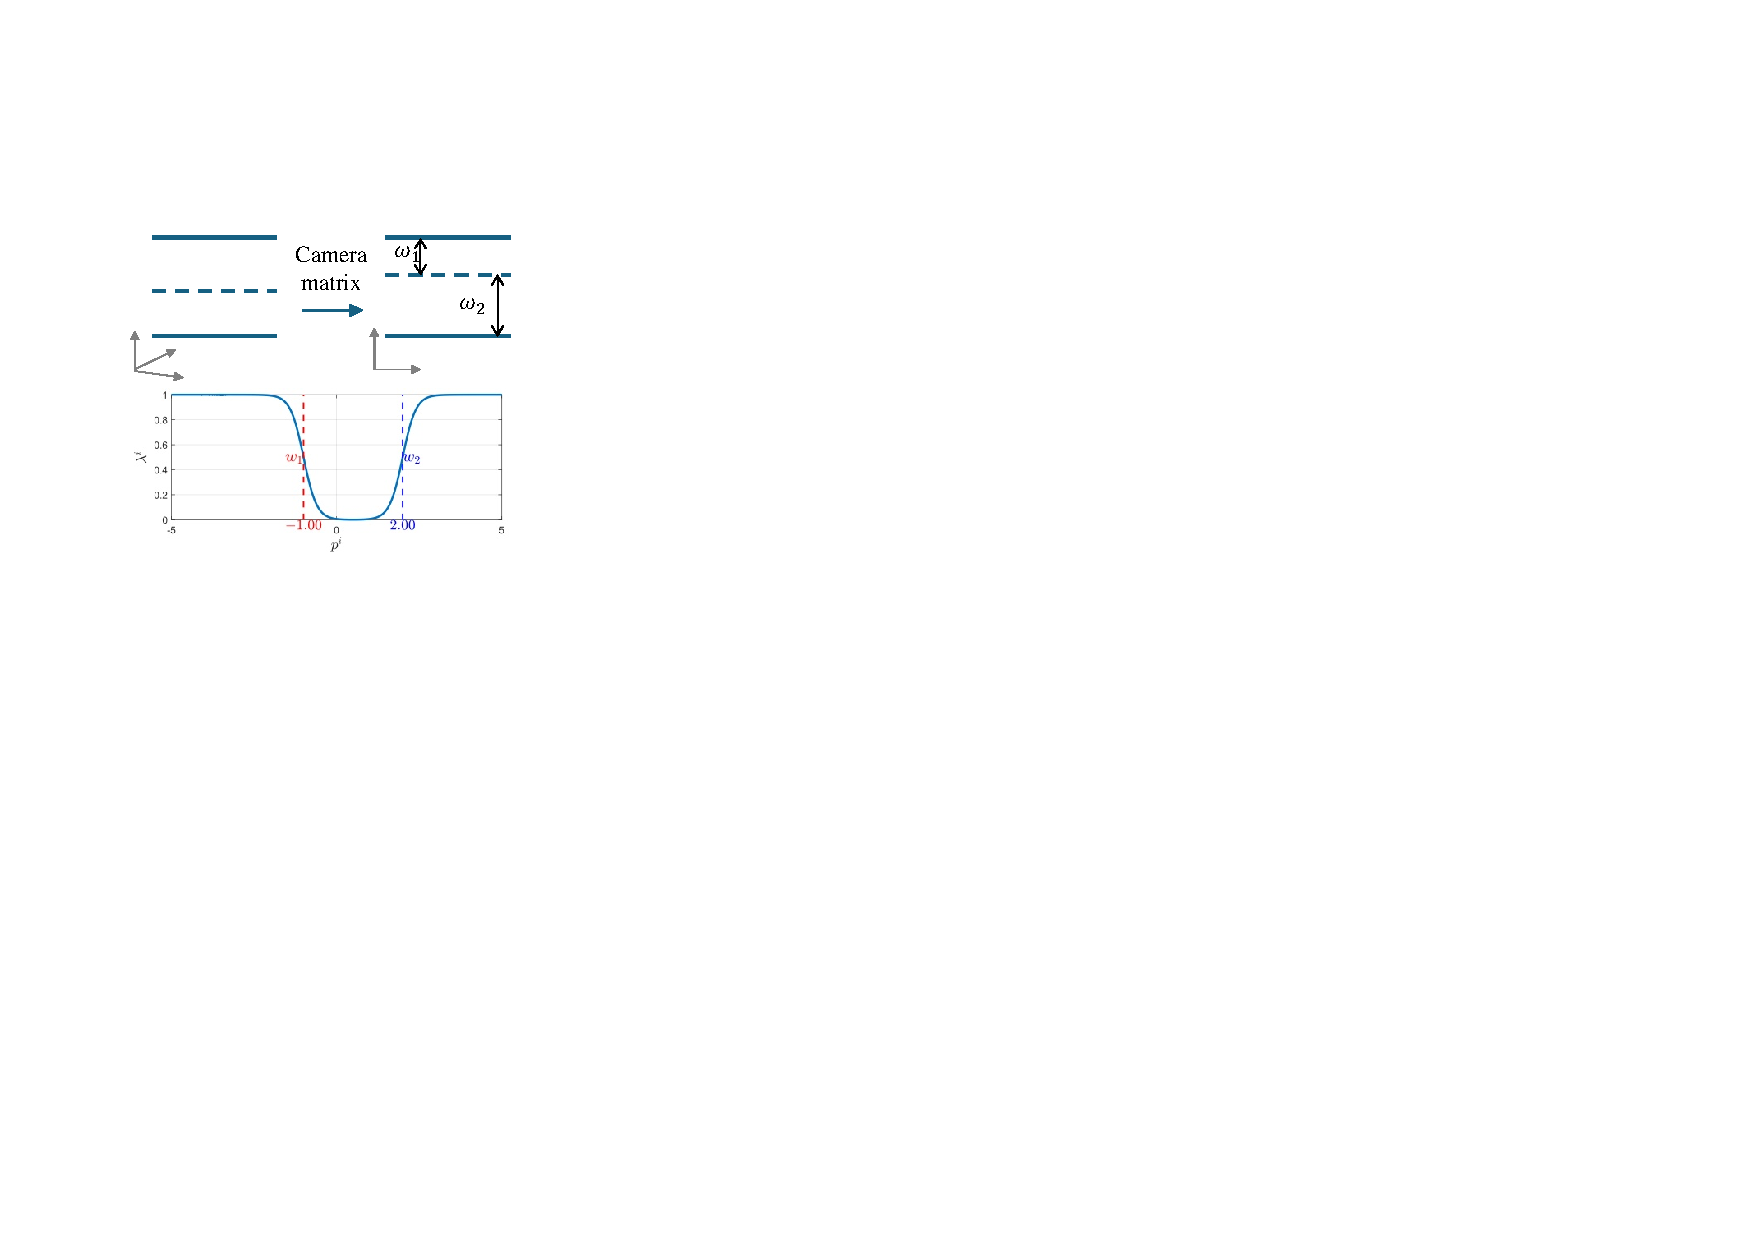
\includegraphics[width=0.2\textwidth]{images/linereconstruction1.pdf}
    }
    \hfill % 空格,均匀分布
    % 第二个子图
    \subfloat[Examples of 2D line pairs ]{
        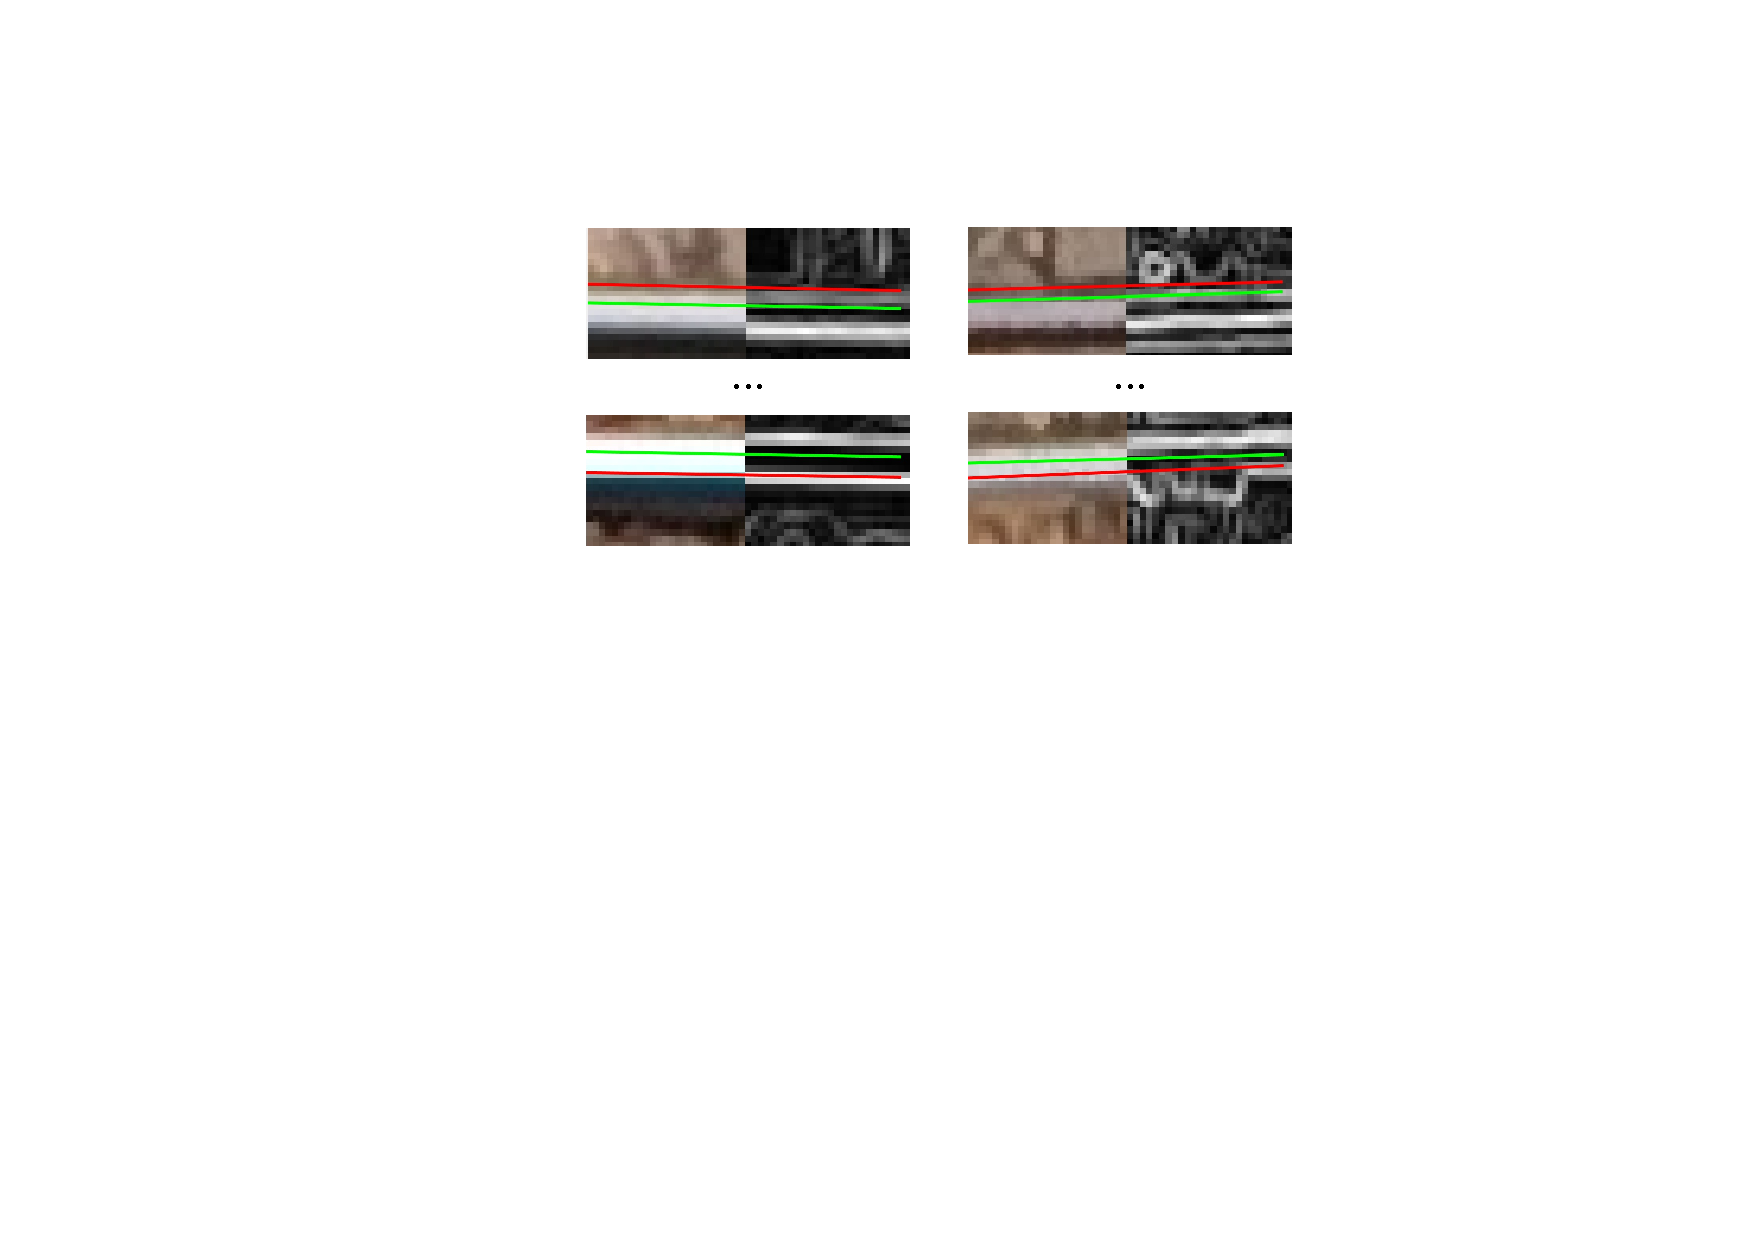
\includegraphics[width=0.40\textwidth]{images/linereconstruction2.pdf}
    }
    \hfill
    % 第三个子图
    \subfloat[The selected 3D line pair with parallel constraint]{
        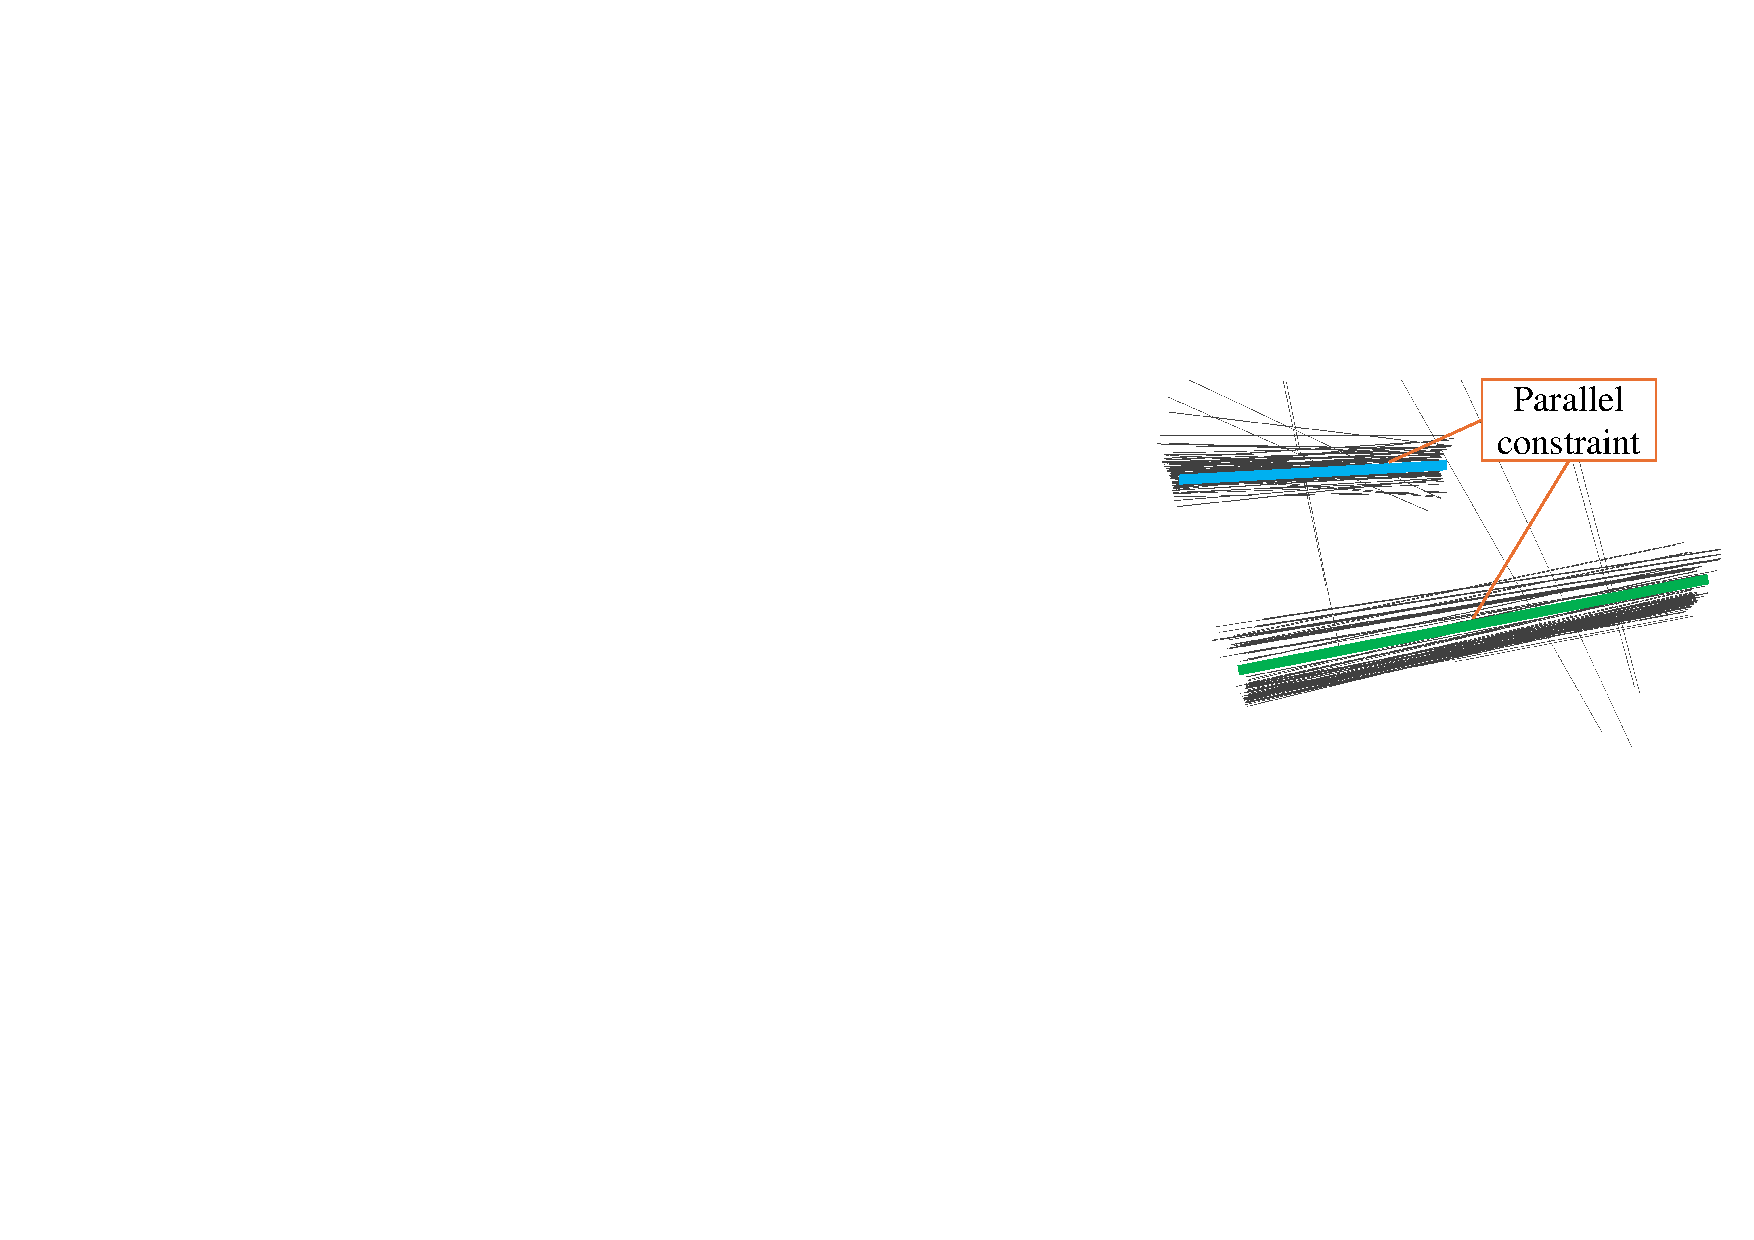
\includegraphics[width=0.35\textwidth]{images/linereconstruction3.pdf}
    }
    \caption{Illustration of the line reconstruction.} % 总标题
    \label{fig:three-images}
\end{figure}


\subsection{Railway reconstruction}
\label{sec_linereconstruction}
In each step of the Kalman process,
the 2D \textit{RL} relating to the prediction of $\bar {\mathbf x}$ can be obtained in images with the camera matrix,
around which the image is slightly extended as the region of interest to find the observation of the 2D \textit{RL}.
We use the tie point in SfM to determine which images the current \textit{RLP} should be projected onto:
we search the $k$ nearest 3D tie points, 
which contain the indices of the images they belong to,
and count the number of tie points associated with each image;
then, 
we select the top $k$ images that contain at least one tie point for 2D \textit{RL} detection.

We use the Hough framework for \textit{RL} detection by converting the Canny edge of the image block into Hough space and constructing the accumulator matrix $\mathrm H$.
Then,
we select the top $k$ peaks in $\mathrm H$ and find the two peaks satisfying 
\begin{equation}
    \begin{aligned}
        &i^*,j^*=\max_{i,j} \left(\mathrm{H}_i + \mathrm{H}_j \right) \\
        &\text{s.t.,} \quad |\theta_i - \theta_j| < t_{ang},
        \quad |\rho_i - \rho_j| < t_{dis2},
    \end{aligned}
\end{equation}
where $\rho_i$ represents the shortest distance between the straight line and the origin of the image coordinate system, while $\theta_i$ is the angle between the straight line and the x-axis.  
The parameter of the distance threshold $t_{dis2}$ is crucial in confirming the railway line,
which determines the width of the railway line that the line will be detected.
As shown in figure 1,
since the railway line has a fixed width in 3D space,
we directly convert it into the image as the distance threshold.
After confirming the two peaks in hough space,
the central 2D line of the railway is fitted by all the pixels subjecting to $i$ and $j$.

In multiple images,
we could find $n_1$ and $n_2$ 2D straight lines for the 3D railway line pair on each side,
and there will be \( n_1 \times (n_1-1) / 2 \) and \( n_2 \times (n_2-1) / 2 \) 3D lines reconstructing from the 2D lines.
Instead of fitting them with least squares,
we select the two representative 3D lines,
which should be parallel and have enough support lines.
It can be formulated as
\begin{equation}
    \begin{aligned}
        &i^*,j^*=\max_{i,j} \left(S\left(L_i\right) + S\left(L_j\right) \right) \quad \text{s.t.,} \quad \angle \left(L_i,L_j\right)<t_{ang} \\
        &S\left(L\right) = \sum \mathcal{N}\left(d(L,L_i), \mu, \left(t_p/3\right)^2\right)
    \end{aligned}
    \label{eq_3dlinescore}
\end{equation}
When the 2D railway line is unobserved and there are few 3D lines in the reconstruction
the highest score in \cref{eq_3dlinescore} is likely to be zero,
for which we say the degenerate reconstruction occurs and the Kalman filter will be terminated.


    








